\autsubsection{Polypropylene foam}{Paul Connetable}

\subsubsection{Capabilities of polypropylene foam}

Another possibility for anchoring the penetrator to the ice layer is to use polypropylene foam. Polypropylene foam is a hardening foam, it can be stored at a high pressure and low temperature for a long time. When needed, it is possible to make it expand by increasing its temperature and releasing it into a wider, open space. The expansion of the foam is made thanks to the expansion of a gas contained in the polymer melt. This gas, called blowing agent, creates bubbles in the polymer, which expand and make the foam expand. During the process, the density of the foam lowers, and it crystallizes, becoming harder and rigid.

The concept idea of using a hardening foam to anchor the penetrator to the ice is that the foam can be stored in a ring around the penetrator, like a buoy. When the penetrator needs to be anchored, the foam could be heated up thanks to the heat produced by the RTG, and released in the penetrator's surroundings, by opening apertures in the ring. This way, the foam would expand and crystallize both inside and outside the buoy of the penetrator. The foam could then expand in the hole drilled, and get in contact with the ice matrix. If the ice has asperities or holes, or is slushy, the foam could then follow the ice profile, and offer a resistance to the penetrator descent, by clinging on to the ice.

The polypropylene foams seem to be well suited for our very specific use and the extreme conditions found at the bottom of Europa's ice crust. Moreover, some research has been done in \cite{naguib2002strategies}, to improve drastically some parameters of polypropylene foams. Some of the results found on this study are presented here. In particular, in this paper, the expansion ratio, the foam density in Figure, and the blowing agent pressure are presented for several chemical compositions of the foam in function of the melt temperature. These results are respectively shown here in Figures \ref{foamexpansion}, \ref{foamdensity} and \ref{foampressure}.

\begin{figure}[htb]
\begin{center}
%\fbox{
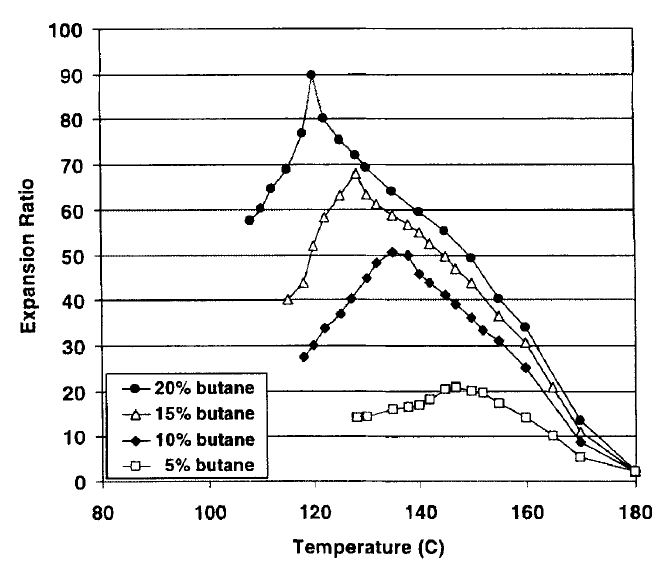
\includegraphics[width=10cm, height=8cm, clip]{figures/Paul/foamexpansion.JPG}
%}
\end{center}
\caption{Expansion coefficients of branched polypropylene material, for different temperatures and material compositions}
\label{foamexpansion}
\end{figure}

\begin{figure}[htb]
\begin{center}
%\fbox{
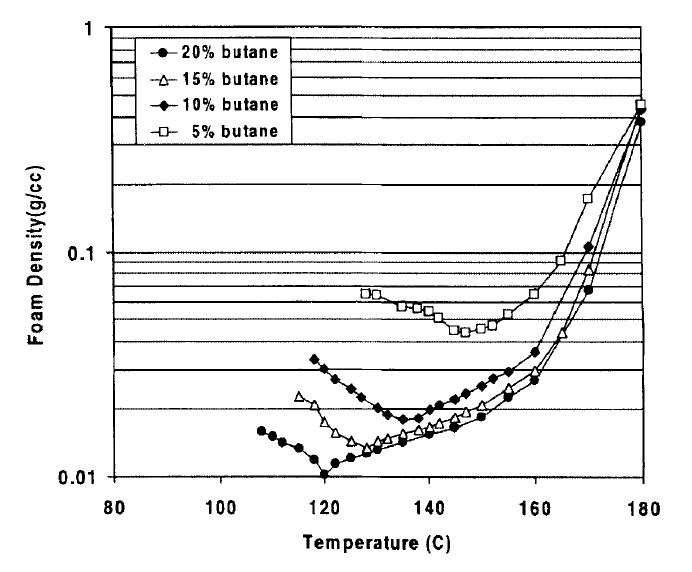
\includegraphics[width=10cm, height=8cm, clip]{figures/Paul/foamdensity.JPG}
%}
\end{center}
\caption{Foam density of branched polypropylene material, for different temperatures and material compositions}
\label{foamdensity}
\end{figure}

\begin{figure}[htb]
\begin{center}
%\fbox{
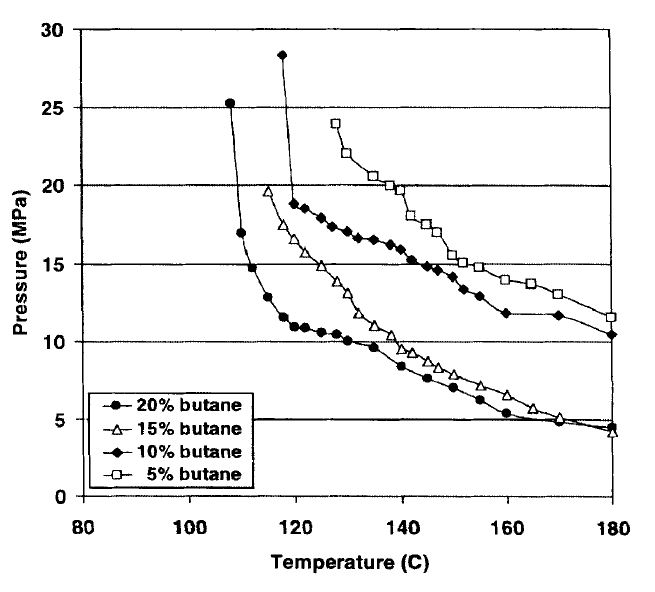
\includegraphics[width=10cm, height=8cm, clip]{figures/Paul/foampressure.JPG}
%}
\end{center}
\caption{Blowing agent die pressure, for different temperatures and material compositions}
\label{foampressure}
\end{figure}


The first interesting result is that, as presented in Figure \ref{foampressure}, the working pressure of the blowing agent in the foam is very high. Even though this working pressure goes down if the butane percentage increases, it is greater than the pressure at 10~km depth under the ice crust on Europa, which is of only about 12~MPa. It means that this kind of foam has a working pressure high enough to still expand in this situation, if the foam temperature is not too high.
Secondly, one can see in Figure \ref{foamdensity} that the foam density is quite low. It is possible to cross this information with Figure \ref{foamexpansion} to find out that the density of the stored product is of about 1 $kg/dm^{3}$, as water. it means that bringing foam would be moderately heavy. However, for reasons explained below, assessing precisely the quantity of foam needed is impossible right now. Finally, as it can be seen in Figure \ref{foamexpansion}, the expansion of the material tested on Earth at 1 bar is very impressive and promising.

\subsubsection{Conclusion on this method}

Anchoring the penetrator thanks to polypropylene foam seems interesting, thanks to some good points of this method. It has indeed the possibility to work at 12~MPa pressure and at the 0°C temperature, thanks to the heat emitted by the RTG. Moreover, since the heat could be obtained thanks to the RTG, it is possible to monitor precisely the temperature of the foam, which is the main variable in its expansion. Since the foam is impermeable, it can be used in water without any problem. It also gives the possibility to anchor in slushy ice, which is not the case of some other methods.


However, it still has some flaws. The most important one is that this anchor could only be used once. This means that it could not be possible to detach the penetrator from its position if the anchoring was not done at the right place, for example if it anchored on the top of lake in the ice crust and not on the ocean. The anchoring would also not be instantaneous but take up to several dozens of seconds to work.
Moreover, no study has been done about anchoring with There is also the possibility that the heated foam could make the ice melt at its contact and therefore, not being able to anchor the penetrator properly.
%Recap of the cons: can be used only once, no research done on this particular use so no value of mass, no security etc


